\section{Dataset and Features}
1. Include a citation on where you obtained your dataset from. 
2. Describe your dataset: how many training/validation/test examples do you have? 
3. Depending on available space, show some examples from your dataset. Try to include examples of your data in the report (e.g. include an image, show a waveform, etc.).
4. What is the resolution of your images? 
5. Is there any preprocessing you did? 
6. What about normalization or standardization? 

The dataset in this study encompasses 525 bird species, featuring 84,635 training images, along with 2,625 images each for testing and validation (5 per species). Rigorous dataset analysis tools were applied to eliminate duplicates and low-quality images, ensuring the dataset's integrity and preventing leakage across train, test, and validation sets.\footnote{Laszewski, G. von. (2023). 100 Bird Species [Data set]. Kaggle. \url{https://www.kaggle.com/datasets/gpiosenka/100-bird-species}}

Each 224x224x3 color image in JPG format, predominantly featuring the bird, is meticulously categorized into 525 folders per species. Accompanying this is a comprehensive CSV file detailing file paths, labels, scientific names, dataset types, and class indices. 
The test and validation images, carefully chosen for their quality, enhance the dataset's robustness. 

The birds in each of the images will take up at least 50\% of the pixels in the image. The images are all gathered from the internet, they where thoroughly chekced for the presence of any duplicated data. This prevent the same images being in the test, validation and train set. 

There is one downside of the dataset, which is the ratio of male species to female species. The dataset contains of around 80\% of male images while only just containing 20\% female images. There is a good reason for it, being that male birds are far more colored, while the female birds are more bland. This makes that the algorithm will be good for detecting the male species but it will struggle giving a accurate classification for the female, because their coloring is more bland. 

For the Neural networks the images where augmented by also including the vertically swapped version of each image. 

\begin{figure}[h]
    \centering
    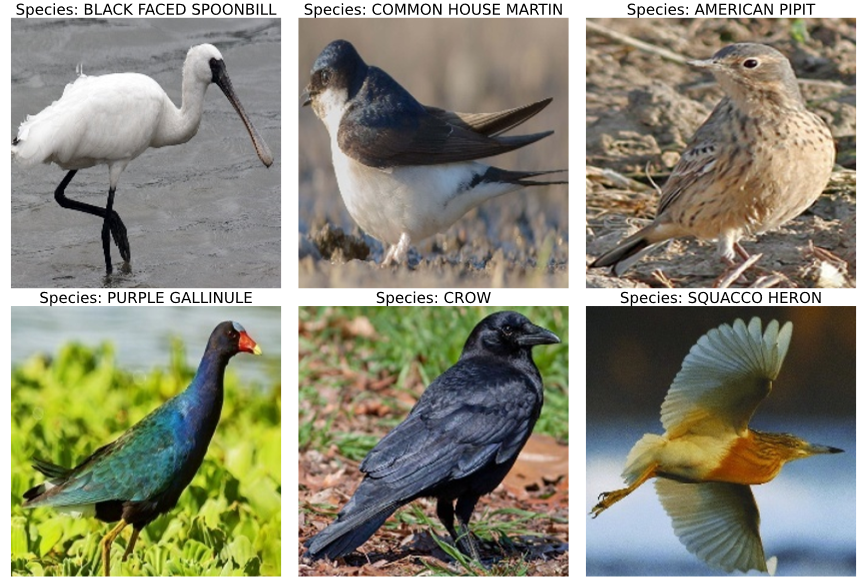
\includegraphics[width=0.5\textwidth]{figs/dataset.png}
    \caption{Images in dataset}
    \label{fig:dataset}
\end{figure}